% \iffalse
\let\negmedspace\undefined
\let\negthickspace\undefined
\documentclass[journal,12pt,twocolumn]{IEEEtran}
\usepackage{cite}
\usepackage{amsmath,amssymb,amsfonts,amsthm}
\usepackage{algorithmic}
\usepackage{graphicx}
\usepackage{textcomp}
\usepackage{xcolor}
\usepackage{txfonts}
\usepackage{listings}
\usepackage{enumitem}
\usepackage{mathtools}
\usepackage{gensymb}
\usepackage{comment}
\usepackage[breaklinks=true]{hyperref}
\usepackage{tkz-euclide} 
\usepackage{listings}
\usepackage{gvv}                                        
\def\inputGnumericTable{}                                 
\usepackage[latin1]{inputenc}                                
\usepackage{color}                                            
\usepackage{array}                                            
\usepackage{longtable}                                       
\usepackage{calc}                                             
\usepackage{multirow}                                         
\usepackage{hhline}                                           
\usepackage{ifthen}                                           
\usepackage{lscape}
\usepackage[center]{caption} % center the captions to figure

\newtheorem{theorem}{Theorem}[section]
\newtheorem{problem}{Problem}
\newtheorem{proposition}{Proposition}[section]
\newtheorem{lemma}{Lemma}[section]
\newtheorem{corollary}[theorem]{Corollary}
\newtheorem{example}{Example}[section]
\newtheorem{definition}[problem]{Definition}
\newcommand{\BEQA}{\begin{eqnarray}}
\newcommand{\EEQA}{\end{eqnarray}}
\newcommand{\define}{\stackrel{\triangle}{=}}
\theoremstyle{remark}
\newtheorem{rem}{Remark}
\begin{document}

\bibliographystyle{IEEEtran}
\vspace{3cm}

\title{NCERT 11.9.5} % TODO: change wrong problem number
\author{ee23btech11223 - Soham Prabhakar More% <-this % stops a space
}
\maketitle
\newpage
\bigskip

\renewcommand{\thefigure}{\theenumi}
\renewcommand{\thetable}{\theenumi}

\bibliographystyle{IEEEtran}

\textbf{Question:}\\
Which term of the following sequences:\\
(a) 2,$2\sqrt{2}$,4\dots is 128
\quad(b) $\sqrt{3}$,3,$3\sqrt{3}$\dots is 729\\
(c) $\frac{1}{3}$,$\frac{1}{9}$,$\frac{1}{27}$\dots is $\frac{1}{19683}$

\textbf{Answer:} (a) Let $a_1 = 2$, $a_2 = 2\sqrt{2}$, $a_3 = 4$.\\
Since, $\frac{a_2}{a_1} = \frac{a_3}{a_2}$, the sequence $a_1, a_2, a_3$ is a G.P Series.
Let $r = \frac{a_2}{a_2} = \sqrt{2}$, then the general term is $a_n = a_1 r^{n-1}$.\\
Assume $n^{th}$ term is 128, which gives: 
\begin{gather*}
    a_n = a_1 r^{n-1} = 128\\
    \implies r^{n-1} = \frac{128}{a_1}\\
    \implies n - 1 = \log_{r}{\frac{128}{a_1}}
\end{gather*}
Substituting Values,
\begin{gather*}
    \implies n - 1 = \log_{\sqrt{2}}{\frac{128}{2}}\\
    \implies n - 1 = \log_{\sqrt{2}}{64}\\
    \implies n - 1 = \log_{\sqrt{2}}{\sqrt{2}^{12}}\\
    \implies n - 1 = 12\\
    \therefore n = 13
\end{gather*}
Thus the $13^{th}$ term of the G.P $a_n$ is 128.\\ 
\[ x(n) = a_1r^{n - 1}u[n] \] where $u[0] = 0$.
Taking the Z - transform:
\begin{gather*}
    X(z) = \sum_{n = -\infty}^{\infty}{x(n) \cdot z^{-n}}\\
    \implies X(z) = \sum_{n = 1}^{\infty}{a_1r^{n - 1}z^{-n}}\\
    \implies X(z) = \frac{a_1}{r}\sum_{n = 1}^{\infty}{r^n z^{-n}}\\
    \implies X(z) = \frac{a_1}{r}(\sum_{n = 0}^{\infty}{r^n z^{-n}} - 1)\\
\end{gather*}
\begin{gather*}
    \implies X(z) = \frac{a_1}{r}(\frac{1}{1 - \frac{r}{z}} - 1)\\
    \implies X(z) = \frac{a_1}{r}(\frac{z}{z - r} - 1)\\
    \therefore X(z) = \frac{a_1}{z - r}\forall { \abs{z} > \abs{r}}\\
\end{gather*}
\[\therefore X(z) = \frac{2}{z - \sqrt{2}}\forall { \abs{z} > \sqrt{2}}\]
with ROC: \[{ \abs{z} > \sqrt{2}}\]

(b) Let $b_1 = \sqrt{3}$, $b_2 = 3$, $b_3 = 3\sqrt{3}$.\\
Since $\frac{b_2}{b_1} = \frac{b_3}{b_2}$, the sequence $b_1, b_2, b_3$ is a G.P Series.
Let $r = \frac{b_2}{b_2} = \sqrt{3}$, then the general term is $b_n = b_1 r^{n-1}$.\\
Assume $n^{th}$ term is 729, which gives: 
\begin{gather*}
    b_n = b_1 r^{n-1} = 729\\
    \implies r^{n-1} = \frac{729}{b_1}\\
    \implies n - 1 = \log_{r}{\frac{729}{b_1}}
\end{gather*}
Substituting Values,
\begin{gather*}
    \implies n - 1 = \log_{\sqrt{3}}{\frac{729}{\sqrt{3}}}\\
    \implies n - 1 = \log_{\sqrt{3}}{\frac{3^6}{\sqrt{3}}}\\
    \implies n - 1 = \log_{\sqrt{3}}{\sqrt{3}^{11}}\\
    \implies n - 1 = 11\\
    \therefore n = 12
\end{gather*}
Thus the $12^{th}$ term of the G.P $b_n$ is 729.
\[ x(n) = b_1r^{n - 1}u[n] \]
Using the previous result, the Z-transform of x(n):
\[X(z) = \frac{\sqrt{3}}{z - \sqrt{3}}\]
with ROC: \[ \abs{z} > \sqrt{3} \]

(c) Let $c_1 = \frac{1}{3}, c_2 = \frac{1}{9}, c_3 = \frac{1}{27}$.\\
Since $\frac{c_2}{c_1} = \frac{c_3}{c_2}$, the sequence $c_1, c_2, c_3$ is a G.P Series.
Let $r = \frac{c_2}{c_2} = \frac{1}{3}$, then the general term is $c_n = c_1 r^{n-1}$.\\
Assume $n^{th}$ term is $\frac{1}{19683}$, which gives: 
\begin{gather*}
    c_n = c_1 r^{n-1} = \frac{1}{19683}\\
    \implies r^{n-1} = \frac{1}{19683 c_1}\\
    \implies n - 1 = \log_{r}{\frac{1}{19683 c_1}}
\end{gather*}
Substituting Values,
\begin{gather*}
    \implies n - 1 = \log_{\frac{1}{3}}{\frac{1}{19683 \frac{1}{3}}}\\
    \implies n - 1 = \log_{\frac{1}{3}}{\frac{1}{6561}}\\
    \implies n - 1 = \log_{\frac{1}{3}}{3^{-8}}\\
    \implies n - 1 = 8\\
    \therefore n = 9
\end{gather*}
Thus the $9^{th}$ term of the G.P $c_n$ is $\frac{1}{19683}$.
\[ x(n) = c_1r^{n - 1}u[n] \]
Using the previous result, the Z-transform of x(n):
\[
    X(z) = \frac{\frac{1}{3}}{z - \frac{1}{3}}
    \implies X(z) = \frac{1 }{3z - 1}
\] with ROC: \[ \abs{z} > \frac{1}{3} \]
\begin{figure}[h!]
    \centering
    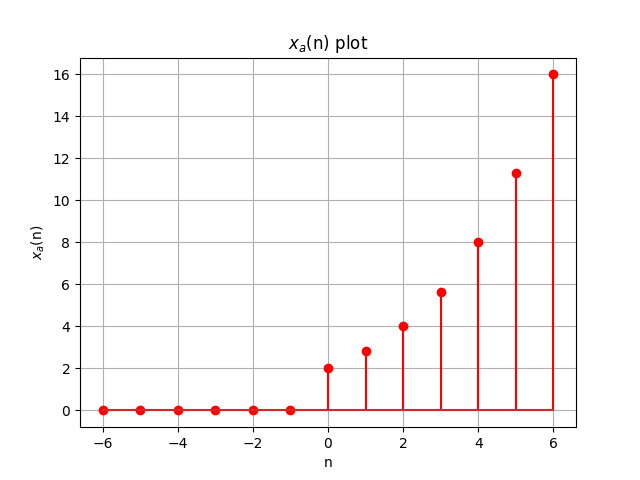
\includegraphics[width=0.5\textwidth]{figs/a.png}
    Fig. 1: Plot of $x_a$(n) from n = -6 to 6
    \label{fig:img1}
\end{figure}

\end{document}

